\documentclass[11pt, A4paper,norsk]{article}
\usepackage[utf8]{inputenc}
\usepackage[T1]{fontenc}
\usepackage{babel}
\usepackage{amsmath}
\usepackage{amsfonts}
\usepackage{amsthm}
\usepackage[colorlinks]{hyperref}
\usepackage{listings}
\usepackage{color}
\usepackage{hyperref}
\usepackage{graphicx}
\usepackage{cite}

\definecolor{dkgreen}{rgb}{0,0.6,0}
\definecolor{gray}{rgb}{0.5,0.5,0.5}
\definecolor{daynineyellow}{rgb}{1.0,0.655,0.102}
\definecolor{url}{rgb}{0.1,0.1,0.4}

\lstset{frame=tb,
	language=Python,
	aboveskip=3mm,
	belowskip=3mm,
	showstringspaces=false,
	columns=flexible,
	basicstyle={\small\ttfamily},
	numbers=none,
	numberstyle=\tiny\color{gray},
	keywordstyle=\color{blue},
	commentstyle=\color{daynineyellow},
	stringstyle=\color{dkgreen},
	breaklines=true,
	breakatwhitespace=true,
	tabsize=3
}

\lstset{inputpath="C:/Users/Torstein/Documents/UiO/Fys1120/Python programmer"}
\hypersetup{colorlinks, urlcolor=url}

\author{Torstein Solheim Ølberg}
\title{Svar på Oblig nr. 2 i Fys1120}



%\lstinputlisting{Filnavn! type kodefil}
%\includegraphics[width=12.6cm,height=8cm]{"C:/Users/Torstein/Documents/UiO/Faget!/Python programmer"/Filnavn! type png}



\begin{document}
	\maketitle
	\begin{center}
		\Large \textbf{Oppgaver}
	\end{center}
	
	
	
	
	
	
	
	
	
		\paragraph{2.}
			\subparagraph{a)}
				\begin{flushleft}
Bruker formelen for kraften fra det magnetiske feltet som er oppgitt i oppgaven og bruker numerisk integrasjon med Euler-Cromer for å finne banen til partikkelen og hastigheten dens. Da får jeg disse plottene:
				\end{flushleft}
					\begin{figure}
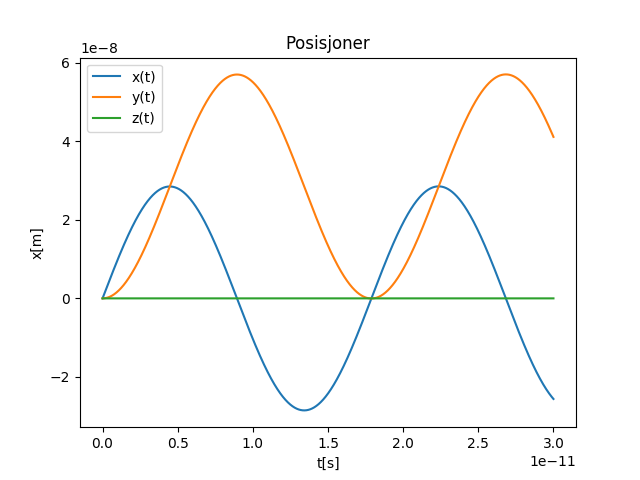
\includegraphics[width=12.6cm,height=8cm]{"C:/Users/Torstein/Documents/UiO/Fys1120/Python programmer"/2a_Posisjoner_2D.png}
\caption{Plott av x, y og z posisjonen til et elektron i B-felt, avhengig av tiden}
					\end{figure}
					\begin{figure}
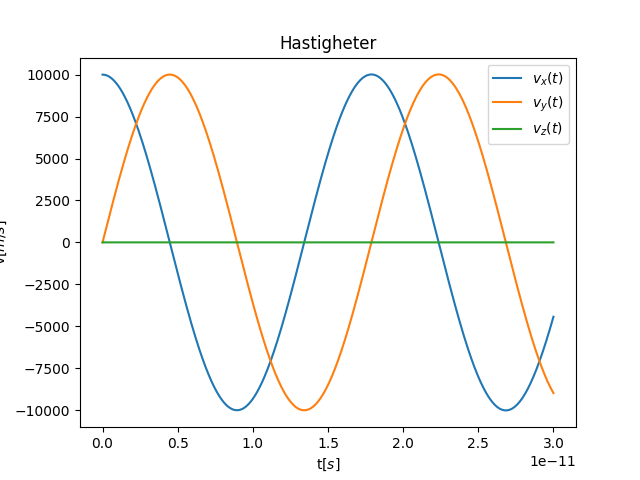
\includegraphics[width=12.6cm,height=8cm]{"C:/Users/Torstein/Documents/UiO/Fys1120/Python programmer"/2a_Hastigheter_2D.png}
\caption{Plott avhastigheten til elektronet i x, y og z rettning i B-felt, avhengig av tiden}
					\end{figure}
					\begin{figure}
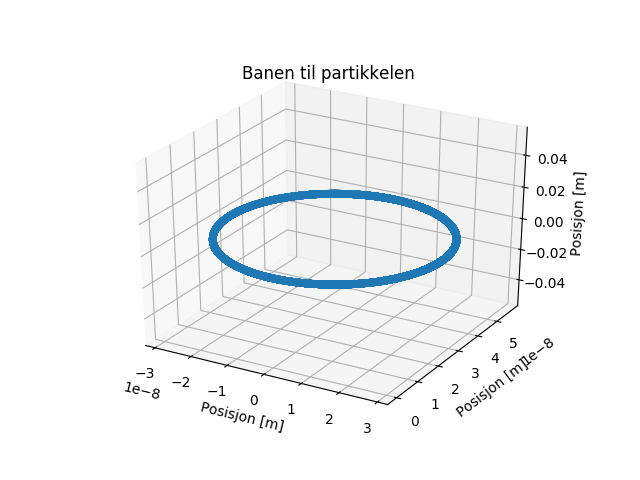
\includegraphics[width=12.6cm,height=8cm]{"C:/Users/Torstein/Documents/UiO/Fys1120/Python programmer"/2a_Posisjoner_3D.png}
\caption{3D plott av elektronet sin bane}
					\end{figure}
\clearpage






			\subparagraph{b)}
				\begin{flushleft}
For å måle omløpstiden la jeg inn en liten test i integrasjonsløkka som printet hvor langt tiden ved det tidspunktet i løkka når alle posisjonene var mindre enn en liten tolleranse på $10^(-10)$. Da fikk jeg 20 forskjellige verdier, og jeg valgte den midterste av de, som var $1.78871924795 \cdot 10^(-11)$
				\end{flushleft}
	
	
	
	
	
	
	
	
	
			\subparagraph{c)}
				\begin{flushleft}
For å bevise dette starter jeg med formelen for kraft som er oppgitt, og bruker sammenhengen mellom hastighet og vinkelhastighet, i tillegg til sammenhengen mellom akselrasjon og vinkelhastighet.
				\end{flushleft}
				\begin{align}
F_B = q(\vec{v} X \vec{B}) \\
a_B = \frac{q(\vec{v} X \vec{B})}{m} \\
\text{Sammenhengene for vinkelhastighet, hastighet,} \nonumber \\
\text{akselrasjon og vinkelakselrasjon:} \nonumber \\
\vec{a} = \vec{\alpha} X \vec{r} + \vec{\omega} X (\vec{\omega} X \vec{r}) = \frac{q((\vec{\omega} X \vec{r}) X \vec{B})}{m} \\
\text{Hverken vinkelhastighet eller B-feltet endrer seg, så $\alpha = 0$} \nonumber \\
\vec{\omega} X (\vec{\omega} X \vec{r}) = \frac{q((\vec{\omega} X \vec{r}) X \vec{B})}{m} \\
\text{Setter inn enhetsvektorer i sylindriske koordinatorer} \nonumber \\
\omega \vec{z} X (\omega \vec{z} X r \vec{r}) = \frac{q((\omega \vec{z} X r \vec{r}) X B \vec{z})}{m} \\
\omega \vec{z} X (\omega r \vec{\phi}) = \frac{q(\omega r \vec{\phi}) X B \vec{z}}{m} \\
- \omega^2 r \vec{r} = - \frac{q \omega r B \vec{r}}{m} \\
\omega_c = \frac{qB}{m} \\
\text{For å bevise neste bruker jeg sammenhengen under:} \nonumber \\
\omega = \frac{2 \pi}{T} \\
\frac{qB}{m} = \frac{2 \pi}{T} \\
T = \frac{2 \pi m}{qB} \\
\text{Regner ut den analytiske omløpstiden:} \nonumber \\
T = \frac{2 \cdot \pi \cdot 9.11 \cdot 10^{-31}}{1.60 \cdot 10^{-19} \cdot 2} sek = 1.78874431714 \cdot 10^{-11} sek \\
\text{Dette er  veldig likt det vi fikk ved numerisk utregning} \nonumber
				\end{align}
\clearpage
	
	
	
	
	
	
	
	
	
			\subparagraph{d)}
				\begin{flushleft}
Endret initialfarten slik som oppgaven sa og fikk en spiral isteden for en ring.
				\end{flushleft}
				\begin{figure}
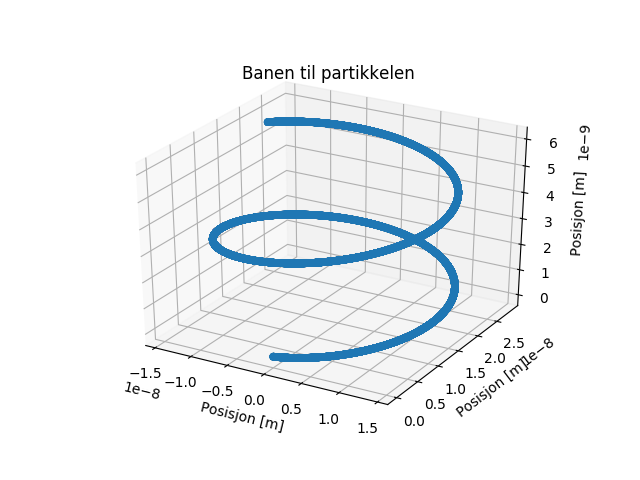
\includegraphics[width=12.6cm,height=8cm]{"C:/Users/Torstein/Documents/UiO/Fys1120/Python programmer"/2d_Posisjoner_3D.png}
\caption{Banen til elektron i B-felt, med initalhastighet i både x- og z-retning.}
				\end{figure}
\clearpage







		\paragraph{3.}
			\subparagraph{a)}
				\begin{flushleft}
Finner kraften fra E-feltet og B-feltet og bruker disse til å regne ut bevegelsen til partikkelen gjennom Euler-Cromer. Satte B-feltet til $1.69T$, og får dette plottet: 
				\end{flushleft}
				\begin{figure}
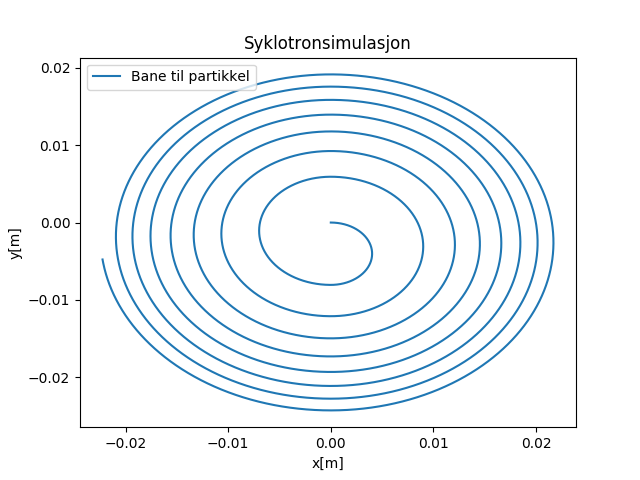
\includegraphics[width=12.6cm,height=8cm]{"C:/Users/Torstein/Documents/UiO/Fys1120/Python programmer"/3a_SyklotronSim.png}
\caption{Simulasjon av proton i syklotron med null B-felt styrke på $1.69$}
				\end{figure}
				\begin{flushleft}
Radien øker ikke like mye i hvert omløp fordi den elektriske kraften er tids- og vinkelfartsavhengig
				\end{flushleft}
\clearpage






			\subparagraph{b)}
				\begin{flushleft}
Legger inn at kraften fra B-feltet slutter ved r = 50mm, og får disse plottene. Satte også simulasjonen til å vare litt lengre siden partikkelen ikke kom helt ut til grensa av syklotronen på tiden gitt i oppgave a.
				\end{flushleft}
\clearpage
				\begin{figure}
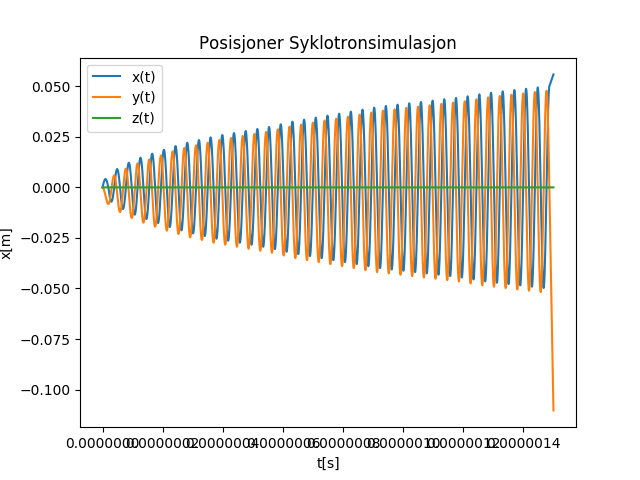
\includegraphics[width=12.6cm,height=8cm]{"C:/Users/Torstein/Documents/UiO/Fys1120/Python programmer"/3b_SyklotronSim_pos.png}
\caption{x, y og z posisjonen til proton i en syklotron}
				\end{figure}
				\begin{figure}
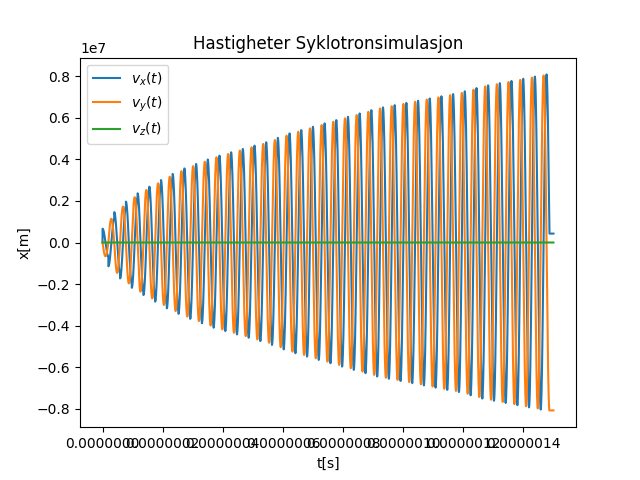
\includegraphics[width=12.6cm,height=8cm]{"C:/Users/Torstein/Documents/UiO/Fys1120/Python programmer"/3b_SyklotronSim_hast.png}
\caption{Hastigheten i x, y og z retning for et proton i en syklotron}
				\end{figure}
\clearpage






			\subparagraph{c)}
				\begin{flushleft}
Farten partikkelen forlater syklotronen med er den samme som den har helt til sist i simulasjonen siden det ikke er noe som gjør noe med partikkelen etter den har sluppet ut. Finner dette ved å finne lengden av den siste hastighetsvektoren.
				\end{flushleft}
	
	
	
	
	
	
	
	
	
			\subparagraph{d)}
				\begin{flushleft}
Bruker formel for kinetisk energi $E_k = \frac{1}{2}mv^2$ og vinkelhastigheten som vi regnet ut i forrige oppgave, i tillegg til sammenhengen mellom hastighet og vinkelhastighet.
				\end{flushleft}
				\begin{align}
E_k = \frac{1}{2}mv^2 \\
\vec{v} = \omega r \vec{\phi} \Rightarrow v = \omega r \\
\omega = \frac{qB}{m} \\
E_k = \frac{m}{2} \left( \frac{qBr}{m} \right)^2 = \frac{1}{2} \frac{q^2 B^2 r^2}{m}
				\end{align}











			\subparagraph{e)}
				\begin{align}
E_k = \frac{1}{2} \cdot \frac{1.602 \cdot 10^{-19} \cdot 1.69^2 \cdot 25 \cdot 10^{-4}}{1.673 \cdot 10^{-27}} = 5.48 \cdot 10^{-14} \\
E_k = \frac{1}{2} \cdot m \cdot v^2 = \frac{1}{2} \cdot 1.673 \cdot 10^{-27} \cdot 8111203^2 = 5.50 \cdot 10^{-14}
				\end{align}	
				\begin{flushleft}
Virker som den er ganske bra for veldig små syklotroner, siden den kinetiske energien er ca. den samme.
Hvis vi utvider syklotronradien til en meter er forskjellen er fortsatt ikke så stor. Har måttet øke $\delta t$ til $10^{-10}$, og forlenge tiden simulasjonen foregår i med en del for at protonet skal komme seg ut da. Når jeg så senker $delta t$ til $10^{-11}$ ser jeg straks at protonet er ganske langt fra å slippe unna, men da tar programmet for lang tid å kjøre til at jeg tør å finne ut hvor lenge simulasjonen må holde på for å bli ferdig.
				\end{flushleft}
				\begin{figure}
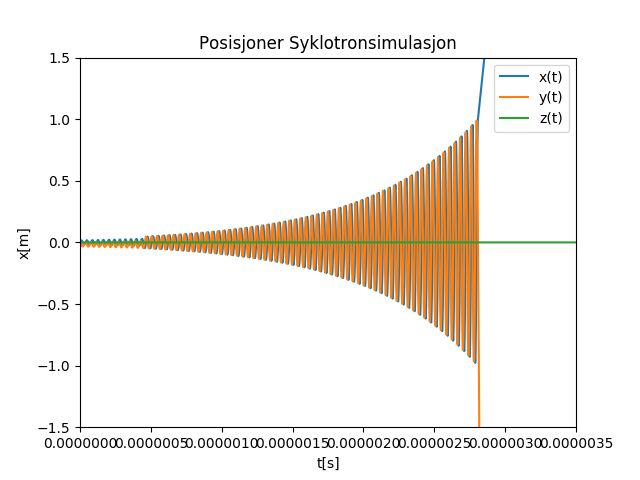
\includegraphics[width=12.6cm,height=8cm]{"C:/Users/Torstein/Documents/UiO/Fys1120/Python programmer"/3e_SyklotronSim_pos.png}
\caption{plott av x, y og z posisjonen, avhengig av tiden, til et proton i en syklotron med radius lik en meter}
				\end{figure}
\clearpage
\lstinputlisting{Oblig2.py}









		\paragraph{4.}
			\subparagraph{a)}
				\begin{flushleft}
Bruker Ampérs lov rundt en sirkelkurve $C$ med radius fra og til: $(0, a), (a, b), (b, b + t), (b + t, \rightarrow)$, altså fire forskjellige sirkler. Alle svarene under er i $\vec{\phi}$ retning.
				\end{flushleft}
				\begin{align}
\int_C \vec{B} \cdot d\vec{l} = \mu_0 I_{\text{total inni $C$}} = \mu_0 \int_S \vec{J} \cdot d\vec{S} \\
\text{B og dl er i samme retning så vi kan fjerne vektorpiler} \nonumber \\
\text{For $r < a$ får vi:} \nonumber \\
J = \frac{I}{\pi a^2} \\
B 2 \pi r = \mu_0 \frac{I}{\pi a^2} \cdot \pi r^2 \\
B = \frac{\mu_0 I r}{2 \pi a^2} \\
\text{For $a < r < b$ får vi:} \nonumber \\
B 2 \pi r = \mu_0 I \Rightarrow B = \frac{\mu_0 I}{2 \pi r} \\
\text{For $b < r < b + t$ får vi:} \nonumber \\
J = \frac{-I}{\pi (b + t)^2}
B 2 \pi r = \mu_0(I + \int_S \vec{J} \cdot d\vec{S}) = \mu_0(I - \left[ \frac{Ir^2}{(b + t)^2} \right]_{b}^{r}) \\
B = \frac{\mu_0 I}{2 \pi r} \left(1 + \frac{b^2 - r^2}{(b + t)^2} \right) \\
\text{for $r > b + t$ får vi:} \nonumber \\
B 2 \pi r = \mu_0 (I - I) = 0 \Rightarrow B = 0
				\end{align}
				\begin{figure}
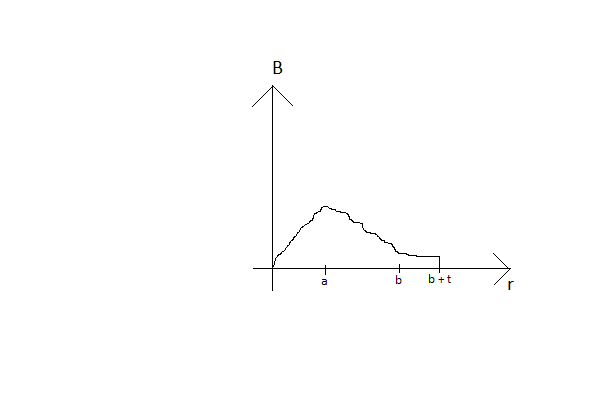
\includegraphics[width=12.6cm,height=8cm]{"C:/Users/Torstein/Documents/UiO/Fys1120/Python programmer"/4a.png}
\caption{Skisse av B-feltet, avhengig av radien $r$}
				\end{figure}
\clearpage









			\subparagraph{b)}
				\begin{flushleft}
Jeg tror det er skisse nummer II. \\
- I og VI er rare fordi de viser et sterkere felt på høyre enn venstre side av den indre lederen, noe som ikke er tilfelle siden den er nærmere ytterlederen der. \\
- III er umulig siden det ikke kan være samme B-feltet inni som utenfor en leder med strøm igjennom seg. \\
- IV er umulig siden feltlinjene starter og stopper ett sted. \\
- V er umulig fordi det ikke kan være et symetrisk felt når innerlederen er forskjøvet fra sentrum.
				\end{flushleft}
\end{document}